\documentclass[a4paper, 11pt, article]{report}
\usepackage[font={small,it}]{caption}
\usepackage[pagestyles]{titlesec}
\usepackage[utf8]{inputenc}
\usepackage{graphicx}
\usepackage{listings}
\usepackage{float}
\usepackage{textcomp}
\usepackage{todonotes}
\usepackage[nottoc,numbib]{tocbibind}

\begin{document}

\titleformat{\chapter}{\bf\huge}{\thechapter}{20pt}{\huge}

%%%%%%%%%%%%%%%%%%%%%%%%%%%%%%%%%%%%%%%%%%%%%%%%%%%%%%%%%%%%%%%%%%%%%%%%%%%%%%%%%%%%%%%%%%%%%%%%%%%%%%%
   
\begin{titlepage}
	\newcommand{\HRule}{\rule{\linewidth}{0.5mm}}
	\center
	
    \textsc{\LARGE Cranfield University}\\[0.8cm]
    
\includegraphics[width=2cm]{images/cranfield}\\[0.8cm]
    \textsc{\Large MSc in Computational and Software Techniques in Engineering 2016/2017}\\[0.8cm]
    \textsc{\large Software Engineering in Technical Computing}\\
    \textsc{\large School of Aerospace, Transport and Manufacturing}\\[1.1cm]
       
    \HRule \\[0.4cm]
    {\huge \bfseries Applications in Practical  \\[0.5cm]
    	High-End Computing}\\[0.3cm]
    \LARGE\HRule \\[1.5cm]
       
    \begin{minipage}{1.1\textwidth}
    	\begin{flushleft} \large
        	{Authors}\\
            Andreas \textbf{Schmidhofer} \\
            Gergő \textbf{Szűcs} \\
            Paweł \textbf{Żybura} \\ 
            Piotr \textbf{Kaźmierczak} \\
            Xin \textbf{Lu}
        \end{flushleft}
    \end{minipage}
	\\[0.9cm] 
    \begin{minipage}{0.9\textwidth}
    	\begin{flushright} \large
        	{Supervisors}
            \\ Dr Dominique \textbf{Fleischmann}
            \\ Dr  Irene \textbf{Moulitsas}
        \end{flushright}
    \end{minipage}\\[1cm]
       
    \vfill
    {\large \today}
    \clearpage
\end{titlepage}

%%%%%%%%%%%%%%%%%%%%%%%%%%%%%%%%%%%%%%%%%%%%%%%%%%%%%%%%%%%%%%%%%%%%%%%%%%%%%%%%%%%%%%%%%%%%%%%%%%%%%%%

\tableofcontents
\newpage

\listoffigures
\newpage

\chapter{Introduction}

In this paper we will discuss the project that we had to complete for the Applications in Practical High-End Computing course, as well as giving \textbf{insight to the team}, the way we had worked throughout the weeks, the \textbf{approaches we took} and the \textbf{results we have achieved}.

The kick-off to the project was five days of introduction to the software, where we had the chance to familiarise ourselves with the concept of the application, its purpose and the source code itself. We were also given many hints and ideas about the possible features and improvements. However, it was emphasised that we were expected to \textbf{think out of the box}, try to \textbf{create something extraordinary}, while still focusing on the feasibility of software for our future customers.

\section{Our vision of the project}

The major idea we had was to \textbf{explore as many aspects of improvement as possible}. First of all, we wanted to apply our already existing software engineering knowledge and everything we had learnt during the Requirements Analysis and System Design course and make sure the source code employs the \textbf{best practices for both efficiency and readability}.

During the first days of the project, we realised that it is a bit cumbersome to set-up the environment and have the code running. Due to that, we wanted to make sure the whole package is as user-friendly as possible, by \textbf{removing} most of the \textbf{third party dependencies}, including them into the deployment and providing a \textbf{standalone installer} for the customers.

Our market analysis had shown that the potential users have troubles using the software. Most of their concerns were about the layout and handling of the graphical interface and the necessity of having three different applications. This put our focus on \textbf{merging two} of the existing \textbf{applications} together and providing convenient access between the remaining two, while also adding quality of life features to the user interface.

Another drawback of the software is the strict requirement of a CUDA-enabled graphics card, which may not be available for many of our customers. Since this is a must because of the complexity of the computations in FlexIT, our idea was to provide \textbf{cloud access to the software} for these customers. In this case, the application would run on a Windows server with a feasible GPU, removing the dependency on the user side.

Creating the meshes in SurfIT was also more complicated than most of the customers would like, and there are many existing applications out there for this task, one of the most famous being CAD. We explored the possibilities of \textbf{importing} the different type of \textbf{models from CAD} into our application, allowing the user to create meshes faster or even use existing ones.

Apart from these ambitious ideas, we also aimed to work on the existing source code, \textbf{implement missing features}, \textbf{fix existing bugs} and in general, \textbf{make the program faster and the user-experience smoother}.

\section{The team}

Our team was based on diversity in both nationalities and expertise. We knew that the project is not only about making the best software but to understand the big picture, \textbf{create an achievable common goal and work towards that as a team}. 

Mixing \textbf{multiple disciplines} in the group helped us a lot to come up with a wide variety of ideas, while the \textbf{cultural diversity} allowed us to learn about the mindset and behaviour of people from different nationalities. As we are in a software engineering course, the majority of the expertise came from this field, while also having a decent amount of mechatronic and  mechanical engineering, as well as mathematics knowledge. Due to the recent Management for Technology course, we were familiar with many aspects of managements, including marketing, which was a big part of the project. \\[0.3cm]

\newpage 

\begin{minipage}{0.3\textwidth}\raggedleft
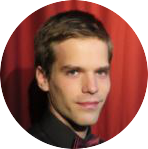
\includegraphics[width=2.5cm]{images/andy}
\end{minipage}
\hfill
\begin{minipage}{0.7\textwidth}\center
Andreas \textbf{Schmidhofer} \\   
Austria \\
Computer scientist
\end{minipage} \\[1.5cm]

\begin{minipage}{0.4\textwidth}\center
Gergő \textbf{Szűcs} \\   
Hungary \\
Software engineer
\end{minipage}%
\hfill%
\begin{minipage}{0.4\textwidth}\raggedright
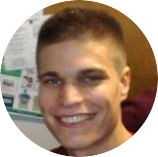
\includegraphics[width=2.5cm]{images/gergo}
\end{minipage} \\[1.5cm]

\begin{minipage}{0.3\textwidth}\raggedleft

\includegraphics[width=2.5cm]{images/pawel}
\end{minipage}
\hfill
\begin{minipage}{0.7\textwidth}\center
Paweł \textbf{Żybura} \\   
Poland \\
Mechatronical engineer
\end{minipage} \\[1.5cm]

\begin{minipage}{0.4\textwidth}\center
Piotr \textbf{Kaźmierczak} \\  
Poland \\
Mechanical engineer
\end{minipage}%
\hfill%
\begin{minipage}{0.4\textwidth}\raggedright

\includegraphics[width=2.5cm]{images/piotr}
\end{minipage} \\[1.5cm]

\begin{minipage}{0.3\textwidth}\raggedleft

\includegraphics[width=2.5cm]{images/xin}
\end{minipage}
\hfill
\begin{minipage}{0.7\textwidth}\center
Xin \textbf{Lu} \\   
China \\
Mathematician
\end{minipage}

%%%%%%%%%%%%%%%%%%%%%%%%%%%%%%%%%%%%%%%%%%%%%%%%%%%%%%%%%%%%%%%%%%%%%%%%%%%%%%%%%%%%%%%%%%%%%%%%%%%%%%%

\chapter{Work organization}

In general, we felt that our group was working quite effectively, keeping in mind that we had assignments and thesis work as well during the group project's period. Every team member was proactive and perceptive during our meetings, while we were also able to work on our own when it was required.
   
\section{Meetings}

During the project all group members had stayed on campus, allowing us to \textbf{meet in person regularly} and sometimes on exceptional occasions. We have held our regular meetings twice a week, usually on Monday and Thursday. On these occasions, we have told each other about the progress we had made, since the previous meeting and discussed the tasks for the next period, while also helping each other with the problems and questions, which we could not solve alone.

We always \textbf{rotated the role of the meeting leader} in our group, to make sure everyone can get familiar with the aspect of it, while also making sure there is always a person to control the flow of these gatherings. The meetings usually took around 30-40 minutes, including the time while we added our notes and tasks to Trello, to make sure we have some footprint of the meeting.

Every now and then some of the group members faced critical problems, which would have caused a delay in our progression, hence they needed to call for \textbf{emergency meetings}. These meetings were not always for the whole group, but for the people who could help the member(s) in need. Thankfully, we did not have too many of these critical situations, and every group member was glad to help each other.
   
\section{External tools}

As we mentioned before, we had used quite a few tools to manage our project. 

\textbf{Trello} was our project management tools, which made handling the tasks and deadlines effortless. We set up different types of lists, where we initially added all our ideas. During our work, we always added the new ideas and bugs to the list, to make sure everyone know about their existence. Then these tasks were assigned to people and given a deadline during our meetings. This allowed us to easily follow what each person was working on at the given time.

To make sure we can follow the dynamic nature of the project and synchronise our work efficiently, we put our source code into a private \textbf{GitHub repository}. This let us share our changes in the source code with each other quickly, and keep track of the changes we made. We could also try out \textbf{experimental features} on branches and merge the promising ones back to the trunk later. Apart from these, it provided us with some interesting feedback on our work, for example, the usual days and hours of commits, the distribution of the programming languages in the code base, etc.

\section{Project timeline}

While our original plan did not exactly come through (due to unexpected issues, new ideas and delays), we have managed to do most of the initial ideas.

\begin{figure}[H]
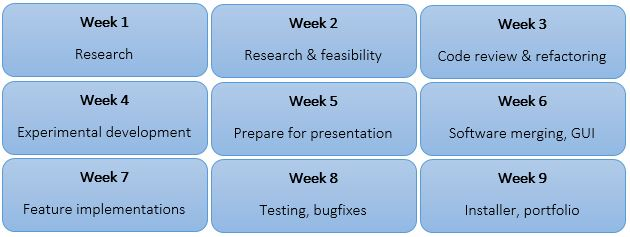
\includegraphics[width=12.8cm]{images/weeklyplan}
\caption{High level initial weekly plan}
\centering
\end{figure}

We will discuss all of the work we carried out in different sections later in this paper.

\section{Individual contribution}

As this was a group project, most of our achievements would not have been possible individually. \textbf{What we have done is the great effort of the whole team}, however here are the parts that each individual mostly worked on. Keep in mind, that we have helped each other in most of the tasks, to allow greater efficiency and faster problem-solving. \\

\noindent Andreas \textbf{Schmidhofer} 
\begin{itemize}
	\item Requirement analysis
	\item Design
	\item Researching cloud computing possibilities
	\item Preparing the presentation
	\item Testing on the Amazon cloud
	\item Creating and editing video for the presentation
	\item Preparing the portfolio
\end{itemize} 

\noindent \\ Gergő \textbf{Szűcs}
\begin{itemize}
	\item Requirement analysis
	\item Design
	\item Code review
	\item Code refactoring
	\item Test plan
	\item Removing third party dependencies
	\item Fixing packaging issues
	\item DesignIT and FlexIT interfacing
	\item Preparing the presentation
	\item Testing 
	\item Graceful handling of errors and exceptions
	\item Bugfixing
	\item Installer creation
	\item Performance measurements
	\item Preparing the portfolio
\end{itemize}

\newpage

\noindent \\ Paweł \textbf{Żybura} 
\begin{itemize}
	\item Requirement analysis
	\item Design
	\item Code review
	\item Merging SurfIT and MoveIT into DesignIT
	\item Command line feature
	\item Preparing the presentation
	\item Merging views to one class
	\item Virtual help tools
	\item GUI redesign
	\item Undo-redo functionality
	\item Testing 
	\item Bugfixing
	\item Preparing the portfolio
\end{itemize}

\noindent \\ Piotr \textbf{Kaźmierczak} 
\begin{itemize}
	\item Market analysis
	\item CAD research
	\item Preparing the presentation
	\item Preparing the portfolio
\end{itemize}

\noindent \\ Xin \textbf{Lu}
\begin{itemize}
	\item Lecture review
	\item Mathematics research
	\item Preparing the presentation
	\item Implementing linear equation solvers
	\item Preparing the portfolio
\end{itemize}

%%%%%%%%%%%%%%%%%%%%%%%%%%%%%%%%%%%%%%%%%%%%%%%%%%%%%%%%%%%%%%%%%%%%%%%%%%%%%%%%%%%%%%%%%%%%%%%%%%%%%%%

\chapter{Research}

We have put a lot of effort into research during our project. Our goal was to make sure we are developing something that is \textbf{wanted by the customers}, \textbf{adds considerable value to the application} and is \textbf{possible} to carry out \textbf{in such a limited time window}. In this chapter, we will present our ideas and the results of the research we had done, while the next chapter will be about the actual development we managed to do.

\section{Market analysis}

To understand what our potential customers would want, we asked some of our colleagues (27 people filled our survey) about their opinion. The survey contained a brief description of the software, what it is made for, how to use it and a download link for the exe file with one JSON file.

Our questions were mainly focused on the interface, whether they like the \textbf{orientation of the GUI}, the \textbf{handling of the software} and if they are satisfied with the \textbf{performance}.

Most of the replies contained concerns about the \textbf{necessity of having three separate applications}. This led us to the decision of \textbf{merging} two of them, as \textbf{SurfIT and MoveIT} were quite similar. We had the feeling that combining FlexIT as well would create and overwhelmingly complicated software, so instead of doing that, we added the functionality which allows the user to \textbf{transfer the current DesignIT project to FlexIT by one mouse click} and return to DesignIT at any time.

Regarding the question, whether they would use the software as it is, we got mixed feedback, but the problem is that we did not receive any details on what they would like us to improve. We have added the command line feature to allow more precise work on the meshes, advanced mouse features for easier camera movement and implemented numerous changes on the interface to make it more user-friendly. We also merged most of the third party dependencies into the program and created an installer which includes the necessary files. This \textbf{allows our users to start working on their project as soon as they receive our application}.

We had other minor feedbacks as well, which we did not have the time to work on, but they should be considered for future development. One of these concerns was the absence of \textbf{supporting multiple file formats for input}. Right now there is no way to import any third-party meshes to the application, which requires the user to learn how to use our program and then possibly the recreation of already existing objects. We have done a lot of research on the possibility of importing objects from AutoCAD, but we did not manage to implement it in time.

Yet another problem was that the \textbf{coefficients} for the simulation \textbf{are} all \textbf{hardcoded} into the program. This seemed to be a small task, but the lack of our knowledge in aeroelasticity and the limited amount of time we had halted the completion of this very useful feature.

About the speed of the program itself, the users were quite satisfied (at least those with better GPUs). However, we still decided to research possible improvements on the algorithms and the CUDA code. For the latter, we did not have enough time, but in general, by merging the two programs, providing an installer, making the user interface easier to use, we possibly saved more time than by improving a bit on the GPU code.

Combining the results from the collected surveys and our experience with the software, we have decided that \textbf{our main goal should be improving the overall user-experience}. The program was already working correctly, and we did not have the necessary knowledge to improve the aeroelasticity part of the code. Instead, we focused on providing a smooth and joyful experience for the customer, while also focusing on researching possible future improvements and granting a considerable speed up, by making the usage of the software easier and the code more efficient.

\section{Mathematics and algorithms}

\subsection{Objective}

After reviewing the slides, one of the ideas of improving the efficiency of the programme was to optimise the algorithm used in computations. Since the efficiency of computation is highly related to the complexity of the algorithm used, optimisation of the algorithm should lead to significant improvement. To reduce the complexity, we studied the original discretization used in the programme to calculate the vector \textbf{V} and studied its implementation, then compared it with other feasible discretizations. On the other hand, we noticed that a linear system has to be solved in the programme, therefore we did research on finding out the proper linear system solver. After the analysis, we implemented the improved algorithm and tested the behaviour.

\subsection{Original method}

First, we did some research about the \textbf{Unsteady Vortex Lattice Method} (UVLM) and analysed the implementation. The discretization considers the lattice over a (wing) surface, and it adopts a labelling scheme where each panel is labelled from 1 to N (the software uses a lattice row and column indexing scheme). These “representative” points are called collocation points, and they are located at the centroid of each panel, and the total velocity potential is the sum the contributions of all the vortex line segments along the edges of all the panels in the lattice. However, the mesh generated doesn't take the thickness of wings into consideration, so we studied other numerical methods to achieve this improvement.

\subsection{Other discretizations}

We modelled the problem, and it can be simplified as solving a partial differential equation, a three-dimensional Laplace equation with one Dirichlet condition (the velocity tends to zero as the distance tends to infinity) and one Neumann condition (the flow is tangential to the surface of the vehicle). To our knowledge, four discretizations were studied.

\begin{itemize}
\item Separation of variables
\item Finite Difference
\item Spectral
\item Finite Element
\end{itemize}

\subsubsection{Separation of variables}

Given that the problem is a three-dimensional partial differential equation, the separation of variables would be very hard. Therefore we have not done any further research about the separation of variables.

\subsubsection{Finite Difference}

The finite difference method is the most common method to solve partial differential equations. In this case, the mesh generation of Finite difference would be difficult because normally the shape of the wings are not regular. Besides, we used the central scheme to calculate the formula expansion and noticed that the computation of next point needs 16 values of previous points, it implies that the communication for parallelization would be huge. Afterwards, we tested an external application using finite difference method, and the performance was not efficient. After discussion, we decided not to implement this method.

\subsubsection{Spectral} 

The conditions of using spectral method are restricted and only a few documents can be found in the library and on the internet. Unfortunately, this method is not suggested for solving Laplace equation according to existing research, therefore we did not focus on spectral method.

\subsubsection{Finite element}

To solve the problem, finite element method subdivides a large problem into smaller, simpler parts that are called finite elements. The simple equations that model these finite elements are then assembled into a larger system of equations that models the entire problem. It is similar to the original UVLM method. However, it can discretize the thickness of wings. For each small, simple part, interpolations will be used to calculate the value. We tried to implement finite element method in the program, however, we would have to change most of \textbf{FlexIT} and also proper interpolation would have to be taken into consideration, therefore we decided to keep the original method and focus on the linear system solver.

\subsection{Linear system solver}

At the end of the computation, a linear system Ax=b will be solved where A is obtained by GPU computation, and b is the known value of the velocity w and the normal vector n. Several methods can be used to solve the linear system, what we have done were studying characteristics of each method and comparing their performance.

\subsubsection{Optimization}

The programme uses Gaussian elimination and LU decomposition to solve the system, which is efficient for a matrix with small size. To gain better performance, we studied other methods and compared them with the original Gaussian elimination.

\begin{itemize}
\item Cholesky method - is effective for a definite positive matrix which is not satisfied in this case.
\item Successive overrelaxation method - works better for huge sparse matrices and it not as effective as Gaussian elimination in this case.
\end{itemize}

\subsubsection{Implementation}

Since our software includes Eigen which provides lots of external functions to solve a linear system, we called function for successive overrelaxation method from Eigen libraries and applied it in our programme. After testing the time consumed, we found out that the Gaussian Elimination is more efficient than successive overrelaxation method.

\section{Cloud computing}

\subsection{Objective}

There are two main goals why we wanted to make FlexIT run in the cloud. First of all, it is one possibility to \textbf{solve the distribution problem}. If you have an image with a working FlexIT installation that can be copied to as many instances as required, then the client does not have to install any software locally but just use those instances. The second goal is to figure out if using different hardware \textbf{change}s the \textbf{performance} of the program. Ideally, if you have a better GPU one would expect that the performance increases. This can be tested with a cloud service because they provide several types of instances which run on different hardware set-up. 

\subsection{Providers}

Currently, there are three big cloud service providers, namely Google with their Google Cloud, Microsoft with Azure and Amazon with \textbf{Amazon Web Services (AWS)}. Google focuses more on Software as a Service (SaaS) and Platform as a Service (Paas), AWS is Infrastructure as a Service (IaaS), and Microsoft does a mixture of PaaS and IaaS. To have the most control and to be able to use the code provided we require IaaS. Therefore AWS is a good choice.

Furthermore, the team has already been working with AWS in the previous project. The university was able to provide an AWS account to cover costs of 40\$, so we were able to use AWS resources. 

\subsection{Implementation}

On AWS we selected the \texttt{g2.2xlarge} instance since it is the cheapest one with a GPU. Additional SSD storage space of 60GB was added because the installation of all the development kits that are required at this stage take up a lot of space. On this instance, we chose Windows Server 2016 Base as an operating system since FlexIT requires Windows. 

Once the instance was started the software could be installed. To allow development we had to install Visual Studio 2015. It is important to install the 2015 version and not a newer version since it the Qt plug-ins are not supported in higher versions. A Qt installation, as well as the appropriate CUDA drivers, had to be installed as well. 

Then the GIT repository could be cloned, and the project opened and executed in Visual Studio. 

\subsection{Results}

The first thing that could be observed is that the graphics were not showing properly. The areas that were supposed to render something just stayed black. This issue could be resolved by \textbf{removing all the OpenGL \texttt{renderText} calls}. 

When running the simulation, the program behaves normally for the first few frames, but then it crashed abruptly. This behaviour was also found on different hardware, for instance, a local computer of one of our colleagues. So it is very likely that it has to do with the hardware. As for now, we were not able to fix this issue. 

No significant runtime difference was found between the execution on AWS and the execution on the lab computer. However, this was just the weakest GPU that AWS has to offer. There are other instance types that support better graphic cards and are specialised on number crunching. 

The biggest problem, however, is that the results that are produced are not correct. In fact, there are no real results produced. The floating point operations return NaN (not a number). This could be tracked down to a part of the software that used CUDA. So maybe there is a problem with the CUDA installation or the GPU. 

\subsection{Conclusion}

We were not able to increase performance by using cloud infrastructure. However, it seems feasible that after the crashing bugs have been sorted out the program could be distributed in this way. Then the customer only needs a Remote Desktop Client and they could \textbf{rent a system on an hourly basis}. 

Future work would be to test the program using a different instance like \texttt{p2.xlarge} which are intended for computing on GPUs. It is possible that the \texttt{p2} instances support CUDA and the \texttt{g2} instances do not. This could solve the NaN problem but in order not to exceed the budget provided we had to stop our investigation.

\section{Importing CAD models}
   
There are many CAD programs, but the most popular program in the world is \textbf{AutoCAD}. It allows you to design two- and three-dimensional coordinate systems and save drawings to a DWG file.

\textbf{DWG} files are a standard for CAD applications. Unfortunately, due to the fact that it is a \textbf{closed binary format reserved by Autodesk}, AutoCAD is required for DWG files. Fortunately, you can also use breaking monopoly programming libraries created by other companies such as Open Design Alliance (formerly OpenDWG).

Autodesk has released some specialised overlays such as AutoCAD Electrical, AutoCAD Mechanical, Mechanical Desktop, Architectural Desktop, and Civil Design that require AutoCAD to be the "engine" that manages their work.

Also, it has provided many programming interfaces for writing custom extensions for AutoCAD.

\subsection{AutoLISP}

It is a variation of the Lisp script language adapted for AutoCAD to automate repetitive operations and increase productivity. For example, calculating the total length of all lines in a drawing - imagine how long it would take to count that.

The great advantage of AutoLISP is that you do not need much programming knowledge to use it. Even a beginner AutoCAD user can create a simple algorithm that will save him hours or days of work.

Another advantage is its portability, as Autodesk did not develop it by moving its attention to another VisualLISP language, it was implemented in the same form in most "clones", so the application written in AutoLISP should equally work in AutoCAD as in IntelliCAD.

\textbf{AutoLISP is a scripting language} which on the one hand can be considered as an advantage (no special programming environment is needed) and on the other hand, it is a big disadvantage, because the scripting language is interpreted during execution, so extensions in it are characterised by slow action.

The entire application code written in AutoLISP is visible to anyone who opens the source code, which is a big minus for commercial programs, no one wants his hard work to be used illegally by others.

In summary, AutoLISP is rather an enhancement for engineers wishing to accelerate the tedious task of writing applications for sale.

\subsection{VisualLISP}

\textbf{VisualLISP} was designed as an extension of AutoLISP functionality. Its capabilities are much more powerful than AutoLISP; it \textbf{has access to the AutoCAD object model}. Besides, the development environment has been implemented in AutoCAD, so developers no longer need to use external editors (as opposed to AutoLISP).

It was introduced in the AutoCAD version 14 as a paid add-on, then later added permanently. But since then, it has been abandoned by Autodesk, which has focused its efforts on more powerful programming interfaces.

VisualLISP as AutoLISP continues to reproduce most of its limitations and are therefore suitable for professional use.

\subsection{DCL}
   
With the help of AutoLISP and VisualLISP, one can not fail to mention the Dialog Control Language (DCL), which makes it easy to build dialogue boxes with simple tags.

DCL has very limited capabilities; no language support is available from the AutoCAD command line.

\subsection{VBA}

Visual Basic for Application is derived from Microsoft Visual Basic and used in many different applications, including AutoCAD. In AutoCAD, it obtains access to objects via the ActiveX interface.

ActiveX Automation was introduced to AutoCAD at the same time as VisualLISP.

No further development of VisualLISP can be attributed to the fact that VBA had the advantage over it in the form of a built-in dialogue box.

In 2007, Microsoft stopped supporting Autodesk in distributing this technology, encouraging developers to use the .NET API.

Autodesk has pushed out unauthorised Microsoft support to 2010, currently no longer has the development environment for VBA, and the language is no longer being developed.

\subsection{ADS}

\textbf{AutoCAD Development System} is a set of libraries written in C language. This interface \textbf{allows you to create applications for AutoCAD in C and C++}.

An external programming environment and programming expertise are needed to create an overlay using ADS.

Compared to previous technologies, the speed of C/C++ programming is increasing significantly, and the possibilities of application development are almost unlimited. You can not only insert parameterized blocks but also "plug" into AutoCAD message loops or overwrite the default functionality of built-in functions.

The big plus of this technology was until recently that most of the "clones" implemented various variants, most of the functions overlapped - so when typing the overlay, it was very likely that without major problems (separate compilation with the appropriate CAD libraries) it will work on AutoCAD and IntelliCAD. Obviously, in the "clones" implementations of subsequent interfaces appear, but they have a long delay compared to Autodesk.

The basic data structure in ADS is resbuf, which contains messages about the type of data contained in it, values written in union form, and a pointer to the next resbuf element.
 
\subsection{ObjectARX}

AutoCAD Runtime eXtension is an API that is the next stage in extending AutoCAD functionality, which includes a set of libraries and C++ header files. All SDKs can be downloaded for free from Autodesk sites.

ObjectARX is the most powerful of all available interfaces, contains all the elements that are available in ADS and develops them with additional functionality.

The performance of this technology is the same as the performance of AutoCAD's functions, and Autodesk's use of AutoCAD extensions such as Autodesk MAP and Architectural Desktop can also be attributed to Autodesk.

Of course, AutoCAD treading on the heels of the competition is trying to make portability portable. Clones based on the DWGDirect library of the Open Design Alliance have the ability to use the ObjectARX-DRX emulation API (e.g., IntelliCAD since version 7, previous versions only implemented ADS).

Some say that ObjectARX is the hardest interface for a programmer although I would bet that it is easier than ADS. However, to get started with it requires knowledge of programming in C ++ and an external development environment (e.g., Microsoft Visual Studio).

\subsection{DWG}
   
DWG - a proprietary binary file format created by AutoCAD. This format was created by Autodesk to support AutoCAD software and derivative programs. Two- and three-dimensional models are written in this format. The owner of the format, Autodesk, distributes it and changes it once every few years with the release of the new version of AutoCAD. DWG format with ASCII variant - DXF has become the de facto standard format for CAD design.

The proprietary format DWG is currently the most used file format in CAD, becoming a standard, without other alternative extended, forcing many users to use this software in a dominant position on the part of the owner company Autodesk.

There exists the OpenDWG library, to access and manipulate data stored in DWG format, which is developed by reverse engineering by an association of manufacturers of CAD software with the intention of supporting their products. As OpenDWG's license does not allow the usage in free software projects, the FSF wants to create an alternative to OpenDWG.

\subsubsection{DWG Support in Freemium and Free Software}

As neither RealDWG nor DWGdirect are licensed under terms that are compatible with free software licenses like the GNU GPL, in 2008 the Free Software Foundation asserted the need for an open replacement for the DWG format. Therefore, the FSF placed the goal 'Replacement for OpenDWG libraries in 10th place on their High Priority Free Software Projects list. Forked in late 2009 from libDWG as GNU LibreDWG project it can read most parts of DWG files from version R13 up to 2004. But as the libreDWG library is released under the GNU GPLv3 it can't be used by most targeted FOSS graphic software, like FreeCAD, LibreCAD and Blender, due to a GPLv2/GPLv3 license incompatibility. 

Due to this struggles in September 2013, the original project LibDWG re-forked its code from LibreDWG. A GPLv2 licensed alternative is the libdxfrw project, which can read simple DWGs. FreeCAD is a free and open-source application that can work with the DWG files by utilising the proprietary Teigha file converter for .dwg and .dxf files from the Open Design Alliance. 

LibreCAD is a free and open-source 2D CAD application that can open DWG and DXF files using your library. Teigha Viewer is a freeware stand-alone viewer for .dwg and .dgn files built on the Teigha development platform from the Open Design Alliance. It runs on Windows, Linux, MacOS and Android operating systems.

Autodesk DWG TrueView is a freeware stand-alone DWG viewer with DWG TrueConvert software included, built on the same viewing engine as AutoCAD software. The freeware Autodesk Design Review software adds a possibility to open DWG files in Design Review to take advantage of measure and markup capabilities, sheet set organisation, and status tracking.

DraftSight is a freemium CAD software from Dassault Systèmes that lets users create, edit and view DWG files. It runs on Linux, Mac and Windows operating systems. 

DWG files can be displayed online by ShareCAD, a free online viewer. This service also offers a free IFrame plug-in for viewing DWG files at a site.

\subsubsection{LibDWG – free access to DWG}

This is a library to allow reading data from a DWG file. That's a very important acquisition, which may improve a lot the ability of the free software community to develop more features in the field of computer technical drawing (CAD).

The DWG structure is very complicated; it seems to be crafted so that none can easily understand it. That's a strong reason not to use it, and that's also why we do not provide the writing feature in the library. One should use LibDWG mainly to read such files, filtering them to some other format, free and usable.

It's easy to figure out the intention to create something like a filter, which takes a DWG file and transforms it to one (or several) of the open alternatives (whenever there be one). It is a long way to reach this goal.
  
\subsection{DXF}
   
It is one of the most popular formats in which you can read 2D as well as 3D elements. Specification of the same template format by Autodesk and a fundamental basis for the exchange of information between AutoCAD and 3D Studio. Over time, the ten format spread and began to be shared by others. Its popularity is related to the copyright related to its sharing in the documentation. DXF is an ASCII text file, so you can improve every save and memorise capability on any hardware and system platform. The downside to this is the relatively large file size compared to its binary DWG counterpart, as well as greater read and write time for the file.
   
The internal organisation of the DXF file is very simple. It consists of pairs of lines in which the odd always contains a "code" defining the meaning of "value" in the next even number. "Code" is always a string that can be converted to an integer. "Value" is a string whose meaning is interpreted accordingly to the preceding "code".
The structure of a typical DXF file consists of the following sections:

\begin{itemize}
\item HEADER - general information about the drawing, can be found in it, such as the name of the program that wrote this file (always on the "code" code of the appropriate meaning and followed by "values").
\item TABLES - a section that describes the special elements of the drawing that have their names and are organised into tables:

\begin{itemize}
\item Linetype (LTYPE) table - An array with line type definitions,
\item Layer table - an array with drawing layer definitions,
\item Text style (STYLE) table - an array with the font type definitions,
\item View table - An array with definitions of saved 3D view settings,
\item User Coordinate System (UCS) table - table with saved locale coordinate system settings,
\item Viewport configuration (VPORT) table - table with drawing window settings (viewports),
\item Drawing manager (DWGMGR) table - table reserved for future use,
\end{itemize}

\item BLOCKS - definitions of drawing blocks, i.e., repetitive elements composed of many basic elements,
\item ENTITIES - the most important section of a file - describes the shape and properties of all the basic elements that comprise the drawing,
\item END OF FILE - end of file tag
\end{itemize}

The above items are specific to drawings created by Autodesk programs. Files from third-party applications often only contain ENTITIES, which is fully acceptable. DXF files saved by AutoCAD sometimes contain data in encoded form. This applies to solids and surfaces created using the Spatial ACIS modelling system, which is part of AutoCAD. This is a clear breakthrough in DXF's "openness" policy so far and has limited access to drawings by third-party programs.

As we have seen, there are many different possibilities to import CAD objects to our program. However, as none of them is convenient, nor efficient, we did not find a good solution to implement in our program, though the research was thorough and we have managed to learn a lot about the existing software and solutions.
   
%%%%%%%%%%%%%%%%%%%%%%%%%%%%%%%%%%%%%%%%%%%%%%%%%%%%%%%%%%%%%%%%%%%%%%%%%%%%%%%%%%%%%%%%%%%%%%%%%%%%%%%

\chapter{Development}

\section{Installer}

After putting a lot of effort on the customer experience, we realised that even if the program is easier to use, if the user has troubles at the beginning while setting up the application, it might affect the overall experience. Hence, we have decided to create a \textbf{standalone installer} for the application. It can be found in the GitHub repository, as well as the submitted code package.

The setup file deploys both programs (DesignIT and FlexIT) to a selected location, and it will also create two shortcuts on the Desktop for them if requested. To make sure the user does not have to install any third party software to run our applications, we are \textbf{providing all the necessary DLL} (Dynamic Linking Library) \textbf{files} within the package. This means after the installation is finished, \textbf{the user can run the program without having to install or configure anything} else.

The package includes the following DLL files.

\begin{itemize}
\item qwindows.dll
\item cudart32\_80.dll
\item Qt5Core.dll
\item Qt5Gui.dll
\item Qt5Network.dll
\item Qt5OpenGL.dll
\item Qt5Widgets.dll
\end{itemize}

\begin{figure}[H]
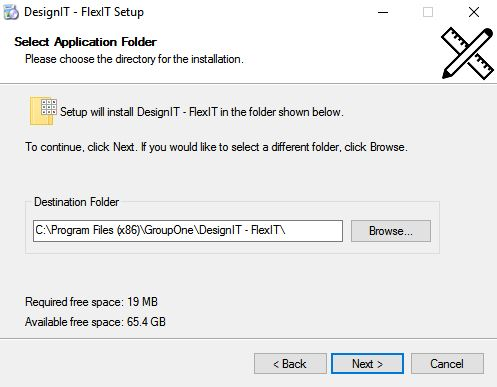
\includegraphics[width=13cm]{images/setup}
\caption{The installer of the software}
\centering
\end{figure}

\section{Code refactoring}

The major problem we had with the source code was \textbf{inconsistency}. Throughout the code, we saw different coding styles, lots of redundant codes and unnecessary comments, which made us spend more time on understanding the code base. During this period, we have tried our best to reformat the code. To do so, we were following the conventions described in \textbf{Google's C++ style guide} [6]. 

The first step was to reorganise the projects. Initially, we had three separate projects, we moved them under \textbf{one solution}, so they can share settings and dependencies (later we also merged two of these project, namely SurfIT and MoveIT into DesignIT), while also allowing us to access them more conveniently.

After that, we spent a few days on looking through the source code, while also making it easier to read and shorter, due to \textbf{removing redundant code chunks and functions}. We have managed to reduce the amount of source code by a great amount, while preserving every functionality and also adding many features and bugfixes.

\section{DesignIT}

At the beginning, we decided that three pieces of software, seeing how much they were individually doing, were too much, especially since the "middle" piece of software - MoveIT - was doing considerably less than other two software pieces, while still being equally important. 

We initially made the decision to combine all three pieces of software, but we quickly backed out from that idea and decided to \textbf{merge} only \textbf{SurfIT and MoveIT}. From that merge new software called \textbf{DesignIT emerged}. DesignIT combines functions of its parents, while at the same time it builds on them and expands. 

Furthermore DesignIT keeps place originally belonging to SurfIT in work pipeline of *IT software, since it's loads files formatted like for SurfIT and outputs files formatted in same way as MoveIT, additionally since SurfIT outputted files with movement data, files outputted by DesignIT could be used in MoveIT and any software that would utilize files at that point *IT work pipeline. The only difference between DesignIT and SurfIT output files is that the second outputted hardcoded dummy movement data, while the first outputs actual user defined data.

\subsection{GUI improvements}

In the case of the main window, changes were more or less cosmetic. On the main toolbar, some buttons were added, repositioned and removed to reflect new functions and modifications to existing ones. 

The main part of the window was divided into three areas using splitters. The most left area originally contained only command window, now two more tabs, previously placed on the right side, were added to it. Those contain information about loaded .json file. Below those new command line, a new input box was added (figure \ref{gui_surface}). In the centre, nearly no changes were introduced. In trajectory mode, the central part contains some controls connected with movement simulation (figure \ref{gui_trajectory}). 

The right side of the main window contains all the editing tabs like views, plots and spreadsheets, divided into surface and trajectory parts using a toolbox. \textbf{The idea behind the new GUI was to split the main window into two clear parts, information part} (left side) \textbf{and work side} (centre and right side). The other idea was only to show tools when they are required.

Regarding user experience, not much have changed with GL widgets used to display all program data. The biggest change is the addition of the new camera controls that allows the user to freely move the camera with mouse only. The rotations are done by holding left mouse button, translations - right, and zoom by using the mouse wheel. At the same time the original controls were mostly left unmodified, so "ctrl" still allows for precise camera movement, and arrows can be used for translations. The same cannot be said for original zoom method (using "shift" key) which was removed.

In the case of the code, our changes are more apparent. First of all, the three widgets that originally were used to display \textbf{2d views of the model were converted into one class} with different drawing methods, depending on the plane they are supposed to represent. This change allowed us to easily implement all the methods that were previously working only on XY view to all 2d views. 

The second big change regarding the code was completely changing the way of how the camera movement was being handled. Changes were done to orthographic projection since those are handled in OpenGL, using a stack of matrices, and it created strange bugs whenever OpenGL's matrix-based functions were called. This method was replaced by the standard method of transforming draw area using translation, rotation and scaling matrices. Currently, all OpenGL widgets use this method of handling camera movement.

\begin{figure}[!h]
	\centering
	
	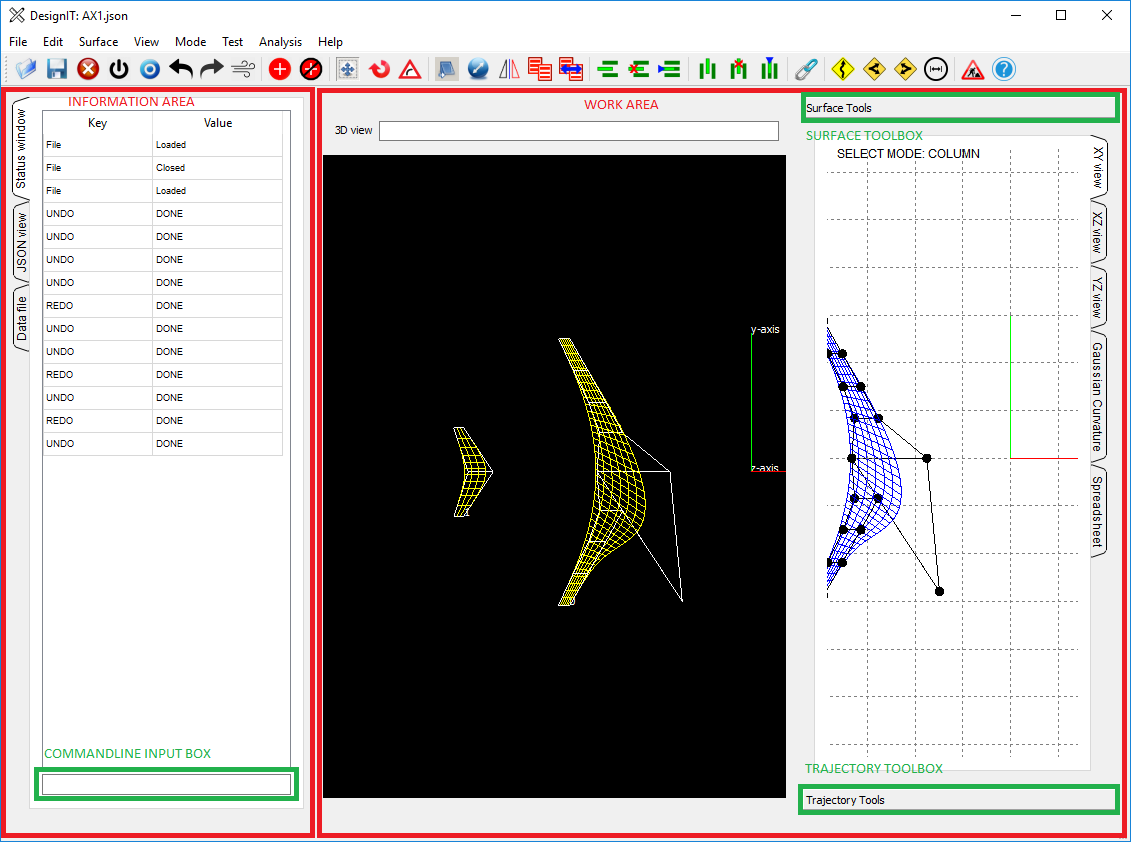
\includegraphics[width=\textwidth]{images/main_window.png}
	
	\caption{Main window with the most important features highlighted}
	
	\label{gui_surface}
\end{figure}

\begin{figure}[!h]
	\centering
	
	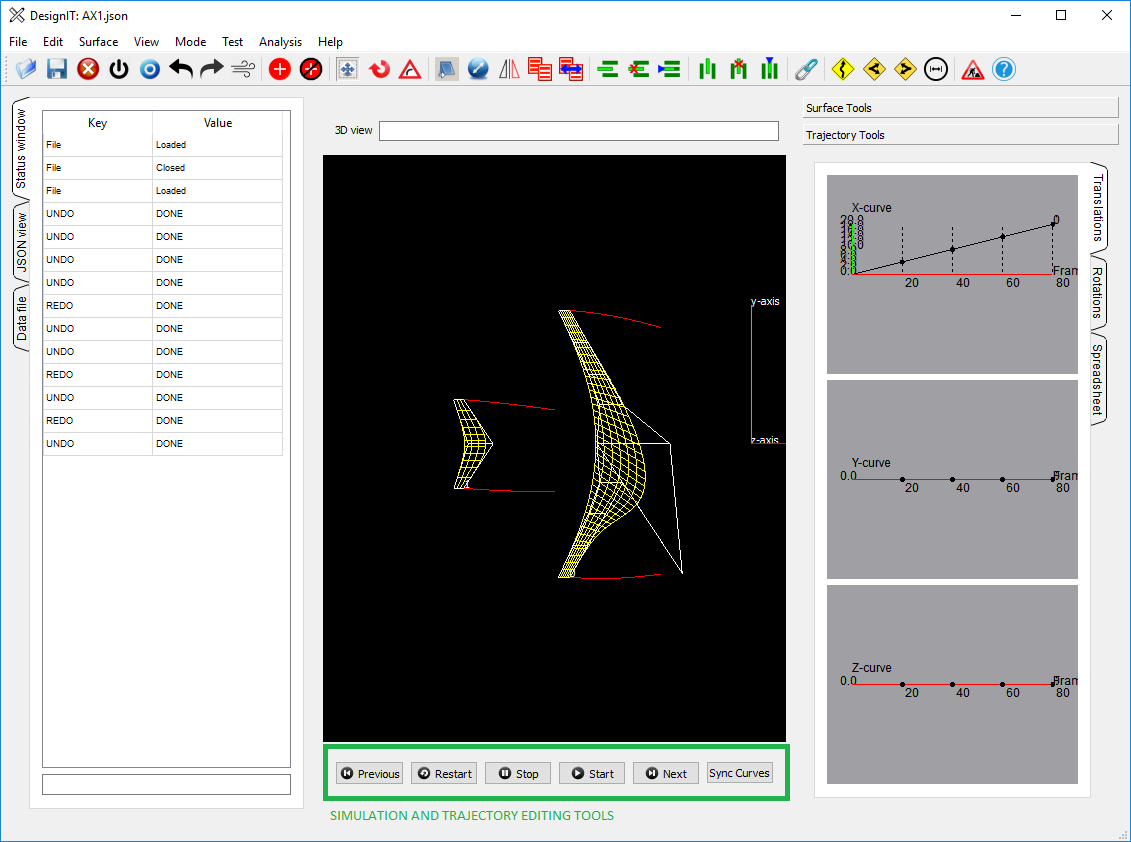
\includegraphics[width=\textwidth]{images/trajectory_window.png}
	
	\caption{Main window in trajectory mode}
	
	\label{gui_trajectory}
\end{figure}

\subsection{Command line}

The command line was an addition inspired by similar solutions found in professional engineering software, for example, AutoCAD. There were two big reasons for including it into DesignIT. Firstly, \textbf{having no command line makes precise editing impossible} (or at least very hard) with only mouse-based controls. The second one was the fact that we wanted to \textbf{base our undo/redo functionality on command system}.

Regarding the code, \textbf{command line system uses a list of keys} (commands) \textbf{and static functions} that are a part of the main window class (DesignIT), stored in the form of a unordered map. The functions (that are called by command names using this map) are responsible for parsing and initial validation of command string, as well as registering proper reverse function on undo/redo stack. The actual transformation is handled by calling the accompanying function that is part of the ITProject class.

Working methods of the ITProject class handle actual command specific transformations. All transformation are handled on the control surface, not accompanying the base surface (base surface are used to write data to file, while the control surface is used for non-permanent transformations). Synchronisation between the two is done only after the command has successfully finished.

\subsection{User help tools}

To make working with the software easier for users, we have included a lot of small features.

\subsubsection{Zoom to cursor}

For all the 2D views we introduced zoom to cursor feature. It means that when the user is zooming - rather than just scaling the view - we also do translations. It makes zooming to a point specified by the user similar to how Google Maps handles zooming.

\subsubsection{Selection modes}

Originally in the program, there were a lot of similar operations differing only in the way data was being selected (for example drag row, drag column). We decided to get rid of those and instead introduce \textbf{selection modes} (figure \ref{highlight_selection}). By using the "alt" key, the user can change the way of how points will be selected. This system offers four modes: point, column, row, surface. It works with dragging, rotating around any point and rotating around the central point of a group of selected points.

\subsubsection{Selection highlight}

To make it easier for users to choose points, we have added a \textbf{highlighting system} (figure \ref{highlight_selection}). If the user puts the mouse cursor close enough to the point he wants to choose, that point will be dynamically highlighted. Furthermore, the system uses selection mode to show the user what he will select (for example, if the surface mode is set and the user is pointing at a point on the surface, the entire surface will be highlighted). This function also spreads to click-based modes to highlight what exactly the operation will be executed on (for example, row in a while using delete row mode).

\begin{figure}[!h]
	\centering
	
	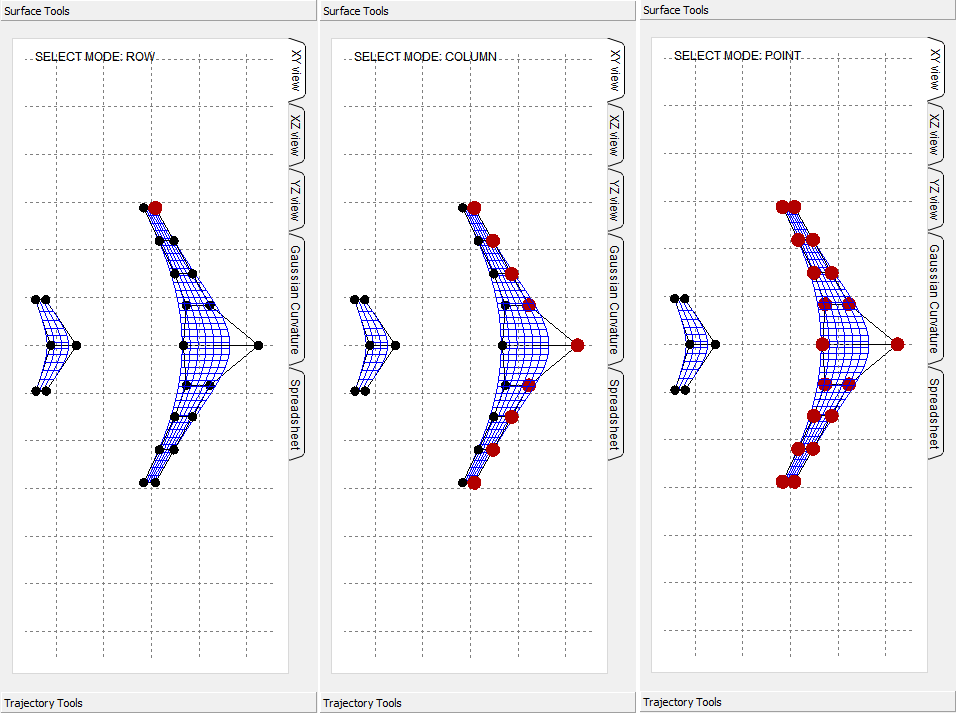
\includegraphics[width=10cm]{images/highlight_feature.png}
	
	\caption{Highlight feature and selection modes. On the left and the centre in drag mode, on the right in surface copy mode}
	
	\label{highlight_selection}
\end{figure}

\subsubsection{Reference point}

Originally the reference point (or as it was called in code scratch point) was used only to store point data for operations that required more than one point to be conducted (i.e. mate points), but this functionality was slightly expanded. \textbf{Reference point is now also drawn} (figure \ref{Reference}), giving user visual reference for a lot of operations (like rotations) since in the code it is also used to determine those operations.

\begin{figure}[!h]
	\centering
	
	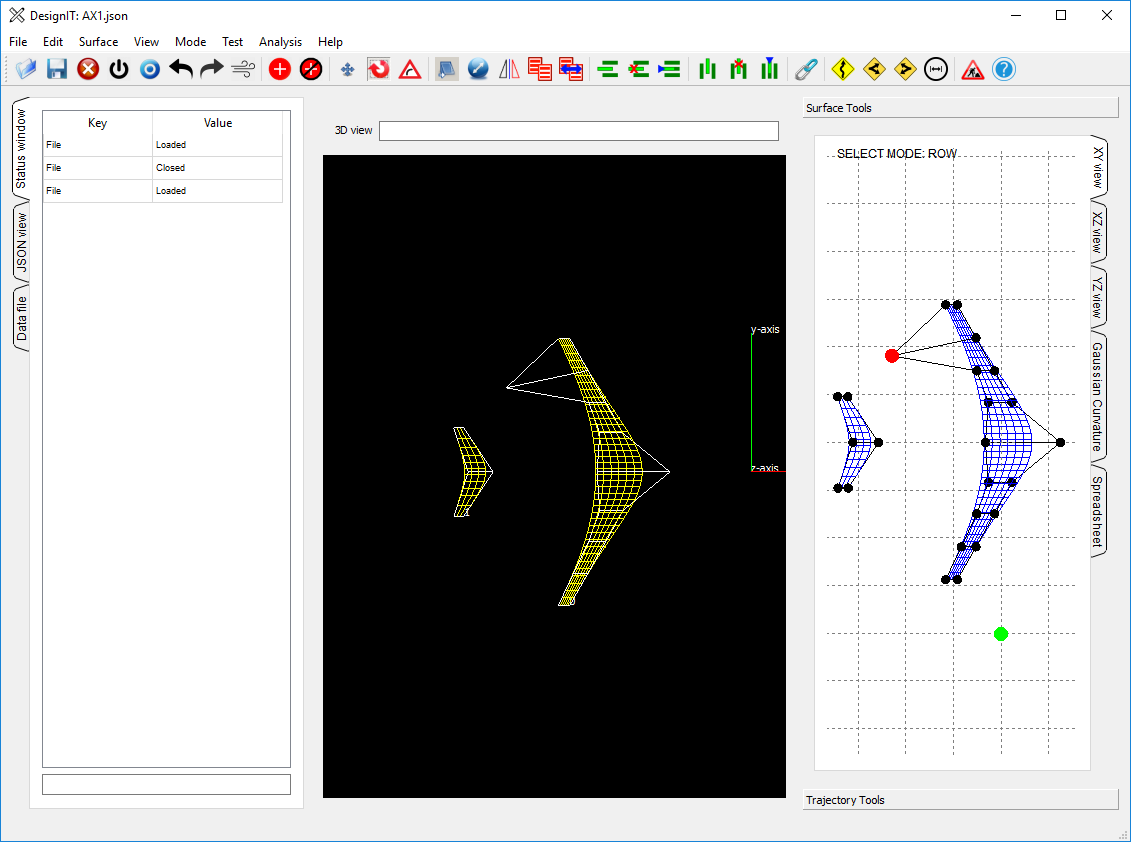
\includegraphics[width=10cm]{images/reference_point.png}
	
	\caption{Reference point in rotation}
	
	\label{Reference}
\end{figure}

\subsubsection{Angle dial}

On top of showing the reference point for rotations, we have introduced a visual device to show the angle which the user have rotated points by and the original position where the rotation started from (figure \ref{angleDial}). Since that kind of help, while useful, might make the view in some situations crowded, so we have given the user the ability to turn it off.

\begin{figure}[!h]
	\centering
	
	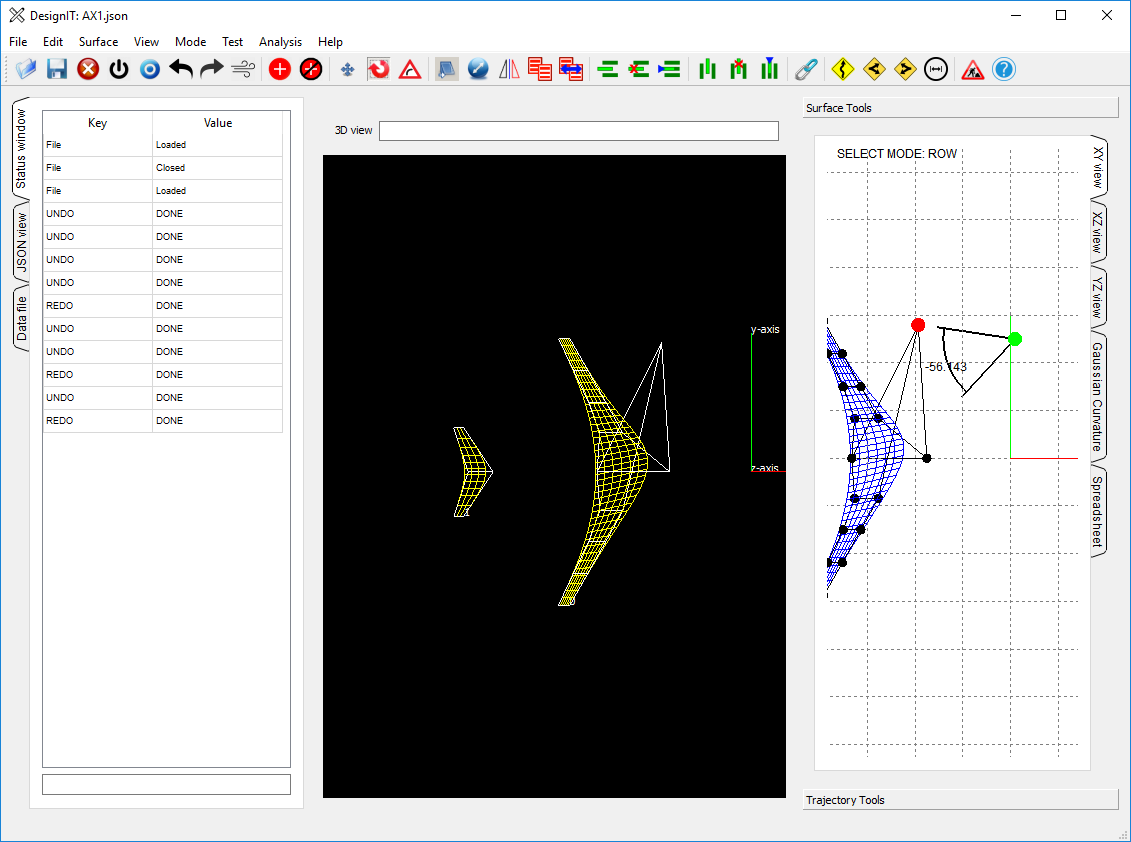
\includegraphics[width=10cm]{images/angle_dial.png}
	
	\caption{Angle dial feature}
	
	\label{angleDial}
\end{figure}

\subsubsection{Drag vector}

To give the user similar kind of help tool for liner transformations as the angle dial is for rotations, we have introduced the drag vector (figure \ref{dragVector}). It is drawn whenever a drag based transformation is handled, similarly to angle dial, it shows origin point (represented by reference point), and values point was dragged in the corresponding plane. As was the case with angle dial, it can also be turned off.

\begin{figure}[!h]
	\centering
	
	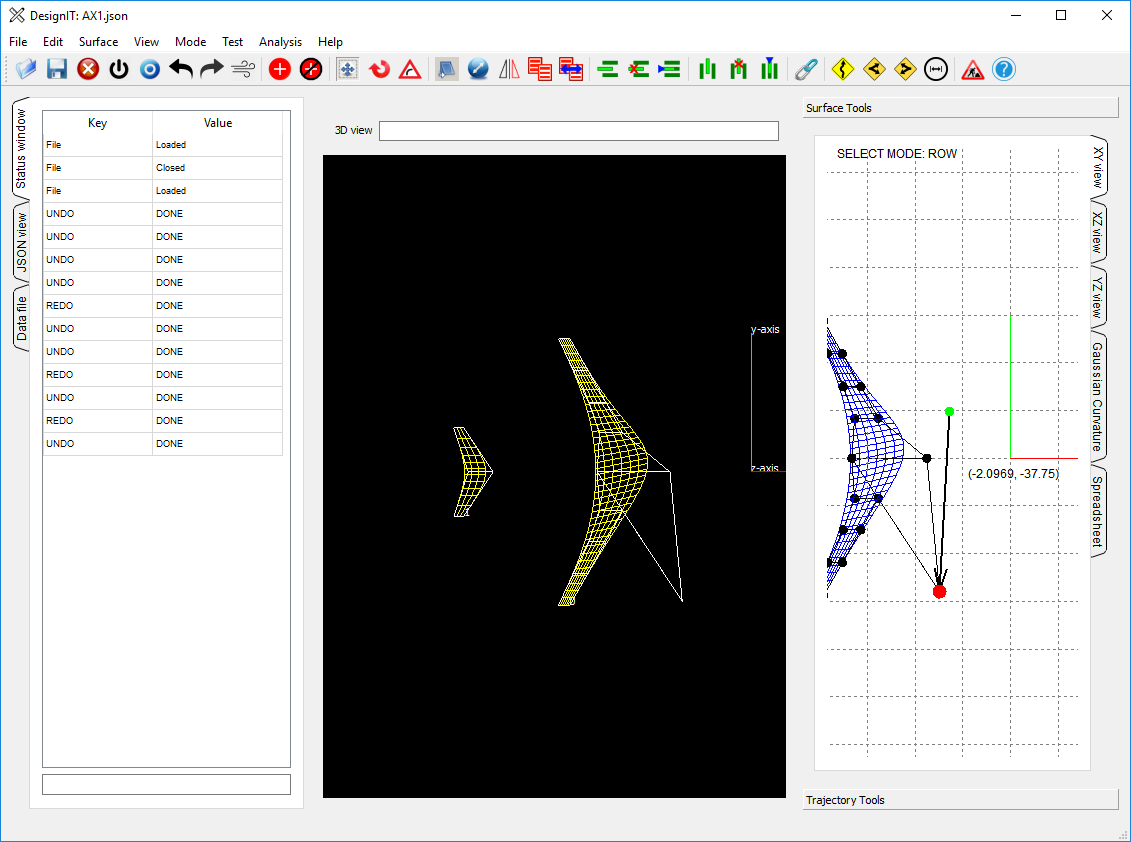
\includegraphics[width=10cm]{images/drag_vector.png}
	
	\caption{Drag vector feature}
	
	\label{dragVector}
\end{figure}

\subsubsection{Trajectory auto edit mode}

In the case of parts of MoveIT that were programmed into DesignIT, we decided to change a little the way MoveIT edit modes were handled. Since there was only one of those and was not conflicting with anything, we have made it activate automatically whenever needed. When the user clicks a trajectory point, edit mode is changed to dragging the trajectory point. It makes using trajectory editing quicker and easier.

\subsubsection{Trajectory sync mode}

Since in many cases aircraft designed in DesignIT will be one plane built from multiple surfaces we decided to make it easier to define a trajectory for all surfaces at once, hence we created sync mode. If it is toggled editing any surface's trajectory curve will also set other the same value for other surfaces.

\subsection{Undo/redo system}

Our undo/redo system uses a command pattern, and \textbf{it is designed to hold all operations from loading the project efficiently}, allowing the user to return to the original state of the system at any moment. Every command line command (if executed with register mode) can create a reverse command. The pair of original commands and reverse commands is saved into the undo/redo stack. Since on the stack one command translates the system from original state to the modified one, and accompanying one from modified to original state, the job of undo/redo system is to keep track of the pointer to the command in this stack, and properly change it on the execution of an undo or redo command. 

This is at least the case for most commands, but there are a few special cases. First of all, delete operations (delete row, delete column, delete surface) are handled differently. Those register special system only undo command on top of the entire deleted entity into undo/redo system. In this case, undo command moves the object from the system's inner bin, back to its original place. This might create problems with memory usage, especially for bigger projects, and when the user does a lot of delete operations. However, since stacks holding removed items are cleared on closing the project, it is not a big problem. 

Another operation that is handled differently is the \textbf{group transformations}. Those are only dragging/rotating by mouse since they have no limitations on the set of points which the user can choose to modify. Those operations register a list of points on which the original transformation was run on and transformation parameters. A special command only runs those transformation on all registered points with one view update.

\subsection{Interfacing between DesignIT and FlexIT}

Another improvement to the DesignIT program is the capability of transferring the current work into FlexIT by one click. 

In the background this process creates a temporary "autosave.json" file, which contains all the data from the current DesignIT project. Using this file, we can launch a new instance of FlexIT to work on the current file. While the user works on FlexIT and checks if the design is working well, DesignIT will keep running in the background. Due to this, if the user finds any problem, he/she can close FlexIT and return to the design phase at any time.

Note that this functionality is only available if there is a project open in DesignIT and also requires the Flexit.exe file to be in the same directory as the Designit.exe application.

\subsection{Other code changes}

On top of these features, a lot of changes were done to the code in general. Many working methods were added to different objects, for example, ITSurface, to make accessing data easier, and also to verify calls (for example throwing an exception on trying to access non-existing surface). Some methods for computations were added, for example calculating the centre of a surface or the centre of a vector of points. Lots of methods were added to ITSurface class, which are accessing methods to rows and columns, used to create copies, adding new or deleting existing ones. 

All those new methods were used in parts of code, that were modified while working on DesignIT, but no full scale redesigning or rewriting the whole code was done, so the original code still uses the old access methods and design choices (for example always keeping copy of a surface in memory, just for the purpose of easily handling dry run). We have upgraded a lot of the code to work better, but still, there is room for improvements.

\section{Bugfixes}

During the development we have fixed numerous bugs in the code, improving the overall user experience by a lot. This is the list of the major bugfixes.

\begin{itemize}
\item Menu icons are not visible in the distributed program
\item The icon of the .exe files are not visible
\item Cancelling the 'Save As' operation results in error
\item Pasting data into table would not update model data
\item GL views affecting each other (strange resizing of window)
\item Removing last row/column with delete mode crash program
\item Modification done in program would not be saved to file
\item Memory leak on deleting column/row
\item Inputting data to spreadsheet would require double conformation to take effect
\end{itemize}

%%%%%%%%%%%%%%%%%%%%%%%%%%%%%%%%%%%%%%%%%%%%%%%%%%%%%%%%%%%%%%%%%%%%%%%%%%%%%%%%%%%%%%%%%%%%%%%%%%%%%%%

\chapter{Testing and results}

We were testing our application throughout the whole development phase, but we also concluded one final testing after we finished working on the code. For the measurement we have used the provided "baseAR4Alpha5deg.json" input data file.

It is important to note, that due to the time limit we had, most of our work was on the user interface, not the performance. However, we still believe \textbf{we have managed to reduce the time the user needs to spend on each project, by making the software easier and quicker to use}.

Our test cases and outcomes can be found in the appendices chapter. Note that wherever applicable the test cases have to be (and they were) \textbf{test}ed \textbf{with their toolbar equivalent button}.

\section{Results}

As we have discussed before, the major speed-up we have achieved is due to the feature we have implemented to the user interface. We did not have enough time to work on the calculations of FlexIT. However, after looking at the code, we have seen some possibilities to improve its performance. We could \textbf{reduce the amount of memory used on the GPU in each consecutive frame}, as there is no need to store the data for every previous step.

Another improvement would be the usage of \textbf{texture memory} in CUDA. Storing the most frequently used data here would result in a high amount of cache-hits, improving the usage of the cache memory and resulting in a possibly major speed-up.

However, we still did the tests with the provided file (baseAR4Alpha5deg) on one of the computers in Building 90. Just to see the the difference between GPUs, we have also tested the same input data on one of our laptops, equipped with an NVIDIA GeForce GTX980M 4GB GDDR5 video card. The comparison is between the calculation time of the last frame (as it takes the most time of all the frames). 

The results were the following for the calculation of the 149th frame in milliseconds.

\begin{center}
\begin{tabular}{ c c c }
 & \textbf{Lab PC} & \textbf{Our Laptop} \\
 \textbf{Dominique's code} & 1332ms & 198ms \\ 
 \textbf{Our code} & 1321ms & 195ms   
\end{tabular}
\end{center}

As expected, the results are quite similar, having only a tiny speed-up in our program. On the other hand, running the code on a stronger GPU gives us \textbf{a speed-up of 6.7}, which is quite good. This also showed us that we made the good decision, to spend more then on the usability of the software, as the CUDA code is quite efficient already. The whole simulation took only 1-2 minutes (depending on the computer), and even if this data was not too complicated, we feel that we have managed to save more time by improving the interface, instead of working on only the performance of the code (surely, if we would have more time, it would have been good to improve the efficiency here as well).

%%%%%%%%%%%%%%%%%%%%%%%%%%%%%%%%%%%%%%%%%%%%%%%%%%%%%%%%%%%%%%%%%%%%%%%%%%%%%%%%%%%%%%%%%%%%%%%%%%%%%%%

\chapter{Conclusion}

We learned a lot of things during the past nine weeks. The best part of the project was \textbf{working with people from different countries and cultures}, while also bringing \textbf{different vision} due to the previous studies we have had. It was interesting to see, what ideas each team member had for development and what we were interested in working on.

The best part was the initial phase, where we could \textbf{freely think and talk about our ideas}, resulting in many great meetings and conversations. After the first few days, however, we had to scrap many of these ideas and focus on those that we decided to be \textbf{valuable and manageable} for this short project.

After the first development phase, we had another fantastic time, while working on the presentation. We have decided to \textbf{make a video about our project}, to have something creative in our presentation, while also creating a lasting memory, which we can watch years later to remember these good times.

Looking back on our work during the weeks, we see that we might have spent more time on research than we should have. However, we think that it was worth the effort. Even though we did not manage to implement many of our good ideas, but we still \textbf{learned a lot of creative ways of solving} those \textbf{issues}.

However, the development we had done is a vast improvement for the program. Combining two of the existing programs into one, and allowing to user to quickly transition between the remaining two will make the life of the future users a lot easier. All the useful features and bugfixes we had discussed in these report, as well as the installer, are also big \textbf{improvements on user-experience}.

Apart from the user side, we worked a lot on the source code itself, making it more readable, shorter and efficient. In overall, we enjoyed working on the project and hopefully carried out satisfying work with great results. \textbf{We would like to thank both Dominique and Irene for your hard work on setting up the project for us and the opportunity itself!}

%%%%%%%%%%%%%%%%%%%%%%%%%%%%%%%%%%%%%%%%%%%%%%%%%%%%%%%%%%%%%%%%%%%%%%%%%%%%%%%%%%%%%%%%%%%%%%%%%%%%%%%

\chapter{Appendices}

\section{Source code - GitHub}

We have sent the source code via e-mail to Dr Moulitsas, but our source code is available on GitHub as well. We had to store it in a private repository for safety reasons, and due to this, an e-mail must be sent to the owner of the repository (g.szucs@cranfield.ac.uk) with a valid GitHub username, to get access to it. 

\section{Project task management - Trello}

As we discussed before, we have used Trello throughout the whole project to manage our work. It is also a private storage, hence the same routine is needed as for GitHub. Please kindly send a valid Trello username to the same e-mail address to be granted access to our project table. 

\section{Common test cases}

\subsection{Install DesignIT \& FlexIT}

\noindent \textbf{Scenario:} Launch the provided setup.exe from the package, select a path for installation and allow the installer to create shortcuts on the desktop.
\\
\noindent \textbf{Result:} The launcher finishes without any errors, the files can be found under the selected location and the shortcuts exist on the desktop.
\\
\noindent \textbf{Status:} \textcolor{green}{Pass}

\section{Test cases - DesignIT}

\subsection{Launch the application}

\noindent \textbf{Scenario:} Launch the exe file using the shortcut located on the desktop.
\\
\noindent \textbf{Result:} The application opens without any errors.
\\
\noindent \textbf{Status:} \textcolor{green}{Pass}

\subsection{Icon visibility}

\noindent \textbf{Scenario:} Check if the shortcut and the exe file have visible icons. Also check whether the menu and toolbar icons are visible in the program.
\\
\noindent \textbf{Result:} Every icon is visible in the program.
\\
\noindent \textbf{Status:} \textcolor{green}{Pass}

\subsection{New}

\noindent \textbf{Scenario:} Click File$\,\to\,$New and make sure the program remains in the new project state. 
\\
\noindent \textbf{Result:} The application did not change.
\\
\noindent \textbf{Status:} \textcolor{green}{Pass}

\subsection{New - unsaved changes}

\noindent \textbf{Scenario:} Add a new surface to an empty project and click File$\,\to\,$New and make sure the program warns you about the unsaved changes. Click "Yes" and verify that an empty project is loaded.
\\
\noindent \textbf{Result:} The application gives a warning. By clicking "Yes" it loads the empty project without saving, by clicking "No" it remains in the original state and allows the saving of the project.
\\
\noindent \textbf{Status:} \textcolor{green}{Pass}

\subsection{Open}

\noindent \textbf{Scenario:} While having an empty project, click File$\,\to\,$Open and select a valid JSON input file. Verify that the data is loaded correctly.
\\
\noindent \textbf{Result:} Using the supplied "baseAR4Alpha5deg.json" file the program loaded the data as expected.
\\
\noindent \textbf{Status:} \textcolor{green}{Pass}

\subsection{Open - unsaved changes}

\noindent \textbf{Scenario:} Add a new surface to an empty project and click File$\,\to\,$Open and verify that the program warns you about the unsaved changes and prompts you to open a new project before loading a file.
\\
\noindent \textbf{Result:} The application gives a warning and after clicking File$\,\to\,$New, the file can be loaded properly.
\\
\noindent \textbf{Status:} \textcolor{green}{Pass}

\subsection{Save As}

\noindent \textbf{Scenario:} While having an empty project, click File$\,\to\,$Save As and verify you get a warning, that there is no data to save.
\\
\noindent \textbf{Result:} Clicking the Save Us button resulted in the expected warning message.
\\
\noindent \textbf{Status:} \textcolor{green}{Pass}

\subsection{Save As - unsaved changes}

\noindent \textbf{Scenario:} Add a new surface to an empty project and click File$\,\to\,$Save As. Verify that a file chooser appears, save the file and then open it. Check if the file contains your previous data.
\\
\noindent \textbf{Result:} Both save and load was successful.data
\\
\noindent \textbf{Status:} \textcolor{green}{Pass}

\subsection{Exit}

\noindent \textbf{Scenario:} Click File$\,\to\,$Exit and make sure the program terminates correctly.
\\
\noindent \textbf{Result:} The application exited without problems.
\\
\noindent \textbf{Status:} \textcolor{green}{Pass}

\subsection{Exit - unsaved changes}

\noindent \textbf{Scenario:} Add a new surface to an empty project and click File$\,\to\,$Exit and make sure the program warns you about the unsaved changes.
\\
\noindent \textbf{Result:} The application gives a warning. By clicking "Yes" it terminates the program without saving, by clicking "No" it remains open and allows the saving of the project.
\\
\noindent \textbf{Status:} \textcolor{green}{Pass}

\subsection{Reset all views}

\noindent \textbf{Scenario:} Open a valid JSON file, move the camera and change the view settings, then click "Reset all Views" on the toolbar. Verify that the view returns to the original state.
\\
\noindent \textbf{Result:} The feature works unpredictably, sometimes it returns to the original state, sometimes it yields some intermediate state.
\\
\noindent \textbf{Status:} \textcolor{green}{Pass(partially)}

\subsection{Add new surface}

\noindent \textbf{Scenario:} Create a new project and click "New surface". Verify that the surface appears in the origo.
\\
\noindent \textbf{Result:} The shape is visible.
\\
\noindent \textbf{Status:} \textcolor{green}{Pass}

\subsection{Undo}

\noindent \textbf{Scenario:} From the previous test's state, click the "Drag points" button and change the shape of the surface using one of the views on the right side. After that, click "Undo" and verify that the shape returns to its original form.
\\
\noindent \textbf{Result:} The shape returned to its original form.
\\
\noindent \textbf{Status:} \textcolor{green}{Pass}

\subsection{Redo}

\noindent \textbf{Scenario:} From the previous test's state, click "Redo" and verify that the shape is changed again. Try the Undo - Redo combination a few times and verify it works as expected.
\\
\noindent \textbf{Result:} Both Undo and Redo works properly, even when clicked multiple times.
\\
\noindent \textbf{Status:} \textcolor{green}{Pass}

\subsection{Delete surface}

\noindent \textbf{Scenario:} From the previous test's state, click "Delete surface" and select the surface on the right side, then verify it's deletion.
\\
\noindent \textbf{Result:} The surface was deleted properly, it can be undone as expected.
\\
\noindent \textbf{Status:} \textcolor{green}{Pass}

\subsection{Interfacing with FlexIT}

\noindent \textbf{Scenario:} Create a new project and click "New surface". Verify that the surface appears in the origo, then click "Open the current project in FlexIT". Make sure FlexIT opens with the current project, and DesignIT continues running in the background. Test if FlexIT is working properly, then close it and verify that DesignIT is still functional.
\\
\noindent \textbf{Result:} Everything working as described.
\\
\noindent \textbf{Status:} \textcolor{green}{Pass}

\subsection{Drag points}

\noindent \textbf{Scenario:} Create a new project and click "New surface", then click the "Drag points" button and change the shape of the surface using one of the views on the right side. Verify that the shape of the surface is changed according to your actions.
\\
\noindent \textbf{Result:} The surface was reshaped correctly.
\\
\noindent \textbf{Status:} \textcolor{green}{Pass}

\subsection{Rotate points}

\noindent \textbf{Scenario:} Create a new project and click "New surface", then click the "Rotate points" button and change the rotation of some points using one of the views on the right side. Verify that the shape of the surface is changed according to your actions.
\\
\noindent \textbf{Result:} The surface was reshaped correctly.
\\
\noindent \textbf{Status:} \textcolor{green}{Pass}

\subsection{Centered rotate}

\noindent \textbf{Scenario:} Create a new project and click "New surface", then click the "Centered rotate" button and change the rotation of some points using one of the views on the right side. Verify that the shape of the surface is changed according to your actions.
\\
\noindent \textbf{Result:} The surface was reshaped correctly.
\\
\noindent \textbf{Status:} \textcolor{green}{Pass}

\subsection{Shear}

\noindent \textbf{Scenario:} Create a new project and click "New surface", then click the "Shear" button. Select one point to rotate around on the right side, then click on another one to rotate the model. Verify that the shape of the surface is changed according to your actions.
\\
\noindent \textbf{Result:} The surface was reshaped correctly.
\\
\noindent \textbf{Status:} \textcolor{green}{Pass}

\subsection{Resize surfaces}

\noindent \textbf{Scenario:} Create a new project and click "New surface", then click the "Resize surfaces" button, then select the surface on the right side. Enter the desired scaling value into the input box and verify that the shape of the surface is changed according to your actions.
\\
\noindent \textbf{Result:} The surface was reshaped correctly.
\\
\noindent \textbf{Status:} \textcolor{green}{Pass}

\subsection{Flip surface}

\noindent \textbf{Scenario:} Create a new project and click "New surface", then click the "Flip surface" button, then select the surface on the right side. Choose the desired axis to flip around and verify that the shape of the surface is changed according to your actions.
\\
\noindent \textbf{Result:} The surface was reshaped correctly.
\\
\noindent \textbf{Status:} \textcolor{green}{Pass}

\subsection{Copy surface}

\noindent \textbf{Scenario:} Create a new project and click "New surface", then click the "Copy surface" button, then select the surface on the right side. Verify that a new copy of the surface has appeared.
\\
\noindent \textbf{Result:} The new surface is visible.
\\
\noindent \textbf{Status:} \textcolor{green}{Pass}

\subsection{Copy surface mirror}

\noindent \textbf{Scenario:} Create a new project and click "New surface", then click the "Copy surface mirror" button, then select the surface on the right side. Select the desired axis to mirror around and verify that a new copy of the surface has appeared, mirrored by the desired axis.
\\
\noindent \textbf{Result:} The new surface is visible and mirrored correctly.
\\
\noindent \textbf{Status:} \textcolor{green}{Pass}

\subsection{Insert row}

\noindent \textbf{Scenario:} Create a new project and click "New surface", then click the "Insert row" button, then select a point of the surface on the right side. Verify that a new row is inserted.
\\
\noindent \textbf{Result:} The row has been added.
\\
\noindent \textbf{Status:} \textcolor{green}{Pass}

\subsection{Delete row}

\noindent \textbf{Scenario:} Create a new project and click "New surface", then click the "Delete row" button, then select a point of the surface on the right side. Verify that a new row is deleted.
\\
\noindent \textbf{Result:} The row has been deleted.
\\
\noindent \textbf{Status:} \textcolor{green}{Pass}

\subsection{Duplicate row}

\noindent \textbf{Scenario:} Create a new project and click "New surface", then click the "Duplicate row" button, then select a point of the surface on the right side. Verify that the row is duplicated.
\\
\noindent \textbf{Result:} The row has been duplicated.
\\
\noindent \textbf{Status:} \textcolor{green}{Pass}

\subsection{Insert column}

\noindent \textbf{Scenario:} Create a new project and click "New surface", then click the "Insert column" button, then select a point of the surface on the right side. Verify that a new column is inserted.
\\
\noindent \textbf{Result:} The column has been added.
\\
\noindent \textbf{Status:} \textcolor{green}{Pass}

\subsection{Delete column}

\noindent \textbf{Scenario:} Create a new project and click "New surface", then click the "Delete column" button, then select a point of the surface on the right side. Verify that a new column is deleted.
\\
\noindent \textbf{Result:} The column has been deleted.
\\
\noindent \textbf{Status:} \textcolor{green}{Pass}

\subsection{Duplicate column}

\noindent \textbf{Scenario:} Create a new project and click "New surface", then click the "Duplicate column" button, then select a point of the surface on the right side. Verify that the column is duplicated.
\\
\noindent \textbf{Result:} The column has been duplicated.
\\
\noindent \textbf{Status:} \textcolor{green}{Pass}

\subsection{Mate points}

\noindent \textbf{Scenario:} Create a new project and click "New surface", then click the "Mate points" button, then select a master point of the surface, and another one on the right side. Verify that the second point is merged into the master point.
\\
\noindent \textbf{Result:} The two points have been merged.
\\
\noindent \textbf{Status:} \textcolor{green}{Pass}

\subsection{Gaussian curvature}

\noindent \textbf{Scenario:} Create a new project and click "New surface", then click the "Gaussian curvature" button. On the right side click the "Gaussian curvature" tab and you can see the curvature of the surface.
\\
\noindent \textbf{Result:} The curvature can be seen.
\\
\noindent \textbf{Status:} \textcolor{green}{Pass}

\subsection{Merge surfaces by row}

\noindent \textbf{Scenario:} Create a new project and click "New surface", copy the surface, then click the "Merge surfaces by row" button. Select both surfaces and choose the type of merge and verify its success.
\\
\noindent \textbf{Result:} The two surfaces have been merged.
\\
\noindent \textbf{Status:} \textcolor{green}{Pass}

\subsection{Merge surfaces by row reverse}

\noindent \textbf{Scenario:} Create a new project and click "New surface", copy the surface, then click the "Merge surfaces by row reverse" button. Select both surfaces and choose the type of merge and verify its success.
\\
\noindent \textbf{Result:} The two surfaces have been merged.
\\
\noindent \textbf{Status:} \textcolor{green}{Pass}

\subsection{Measure distance}

\noindent \textbf{Scenario:} Create a new project and click "New surface", then click the "Measure distance" button. Select two different points of the surface and verify that the distance is written to the text box on the top-center of the screen.
\\
\noindent \textbf{Result:} The distance is visible in the input field.
\\
\noindent \textbf{Status:} \textcolor{green}{Pass}

\subsection{JSON view}

\noindent \textbf{Scenario:} Load one of the supplied JSON files and select "JSON view" on the left side. Verify that you can see the structure of the JSON file in a tree view.
\\
\noindent \textbf{Result:} The JSON structure is visible.
\\
\noindent \textbf{Status:} \textcolor{green}{Pass}

\subsection{Data file}

\noindent \textbf{Scenario:} Load one of the supplied JSON files and select "Data file" on the left side. Verify that you can see the structure and content of the JSON file.
\\
\noindent \textbf{Result:} The JSON data is visible.
\\
\noindent \textbf{Status:} \textcolor{green}{Pass}

\subsection{XY view}

\noindent \textbf{Scenario:} Load one of the supplied JSON files and select "XY view" on the right side. Verify that you can see the surface from the correct view.
\\
\noindent \textbf{Result:} The surface can be seen from the correct point of view.
\\
\noindent \textbf{Status:} \textcolor{green}{Pass}

\subsection{XZ view}

\noindent \textbf{Scenario:} Load one of the supplied JSON files and select "XZ view" on the right side. Verify that you can see the surface from the correct view.
\\
\noindent \textbf{Result:} The surface can be seen from the correct point of view.
\\
\noindent \textbf{Status:} \textcolor{green}{Pass}

\subsection{YZ view}

\noindent \textbf{Scenario:} Load one of the supplied JSON files and select "YZ view" on the right side. Verify that you can see the surface from the correct view.
\\
\noindent \textbf{Result:} The surface can be seen from the correct point of view.
\\
\noindent \textbf{Status:} \textcolor{green}{Pass}

\subsection{Surface Spreadsheet}

\noindent \textbf{Scenario:} Load one of the supplied JSON files and select "Spreadsheet" on the right side. Verify that you can see the data of the surface in a table format and also whether it is editable.
\\
\noindent \textbf{Result:} The data appears and can be freely edited.
\\
\noindent \textbf{Status:} \textcolor{green}{Pass}

\subsection{Trajectory tools}

\noindent \textbf{Scenario:} Load one of the supplied JSON files and select "Trajectory tools" on the right side. Verify that you can see the trajectory of the surface (red lines) and if you click "Start" the surface moves in the direction of the line.
\\
\noindent \textbf{Result:} The trajectory behaves as expected.
\\
\noindent \textbf{Status:} \textcolor{green}{Pass}

\subsection{Translations}

\noindent \textbf{Scenario:} Load one of the supplied JSON files, open the "Trajectory Tools" and select "Translations" on the right side. Verify that you can drag the points on any axis and the change is reflected in the trajectory of the surface.
\\
\noindent \textbf{Result:} The points can be dragged and the trajectory changes properly.
\\
\noindent \textbf{Status:} \textcolor{green}{Pass}

\subsection{Rotations}

\noindent \textbf{Scenario:} Load one of the supplied JSON files, open the "Trajectory Tools" and select "Rotations" on the right side. Verify that you can drag the points on any axis and the change is reflected in the trajectory of the surface.
\\
\noindent \textbf{Result:} The points can be dragged and the trajectory changes properly.
\\
\noindent \textbf{Status:} \textcolor{green}{Pass}

\subsection{Trajectory Spreadsheet}

\noindent \textbf{Scenario:} Load one of the supplied JSON files, open the "Trajectory Tools" and select "Spreadsheet" on the right side. Verify that you can see the data of the surface in a table format and also whether it is editable.
\\
\noindent \textbf{Result:} The data appears and can be freely edited.
\\
\noindent \textbf{Status:} \textcolor{green}{Pass}

\subsection{Web help}

\noindent \textbf{Scenario:} Click the "Web help" button and verify that a new browser windows appears opening the website with the documentation to the software
\\
\noindent \textbf{Result:} The documentation appears.
\\
\noindent \textbf{Status:} \textcolor{green}{Pass}

\subsection{About}

\noindent \textbf{Scenario:} Click the "About" button and verify that a windows with data about the authors appear.
\\
\noindent \textbf{Result:} The window appears.
\\
\noindent \textbf{Status:} \textcolor{green}{Pass}

\section{Test cases - FlexIT}

\subsection{Launch the application}

\noindent \textbf{Scenario:} Launch the exe file using the shortcut located on the desktop.
\\
\noindent \textbf{Result:} The application opens without any errors.
\\
\noindent \textbf{Status:} \textcolor{green}{Pass}

\subsection{Icon visibility}

\noindent \textbf{Scenario:} Check if the shortcut and the exe file have visible icons. Also check whether the menu and toolbar icons are visible in the program.
\\
\noindent \textbf{Result:} Every icon is visible in the program.
\\
\noindent \textbf{Status:} \textcolor{green}{Pass}

\subsection{Open}

\noindent \textbf{Scenario:} While having an empty project, click File$\,\to\,$Open and select a valid JSON input file. Verify that the data is loaded correctly.
\\
\noindent \textbf{Result:} Using the supplied "baseAR4Alpha5deg.json" file the program loaded the data as expected.
\\
\noindent \textbf{Status:} \textcolor{green}{Pass}

\subsection{Open - unsaved changes}

\noindent \textbf{Scenario:} Add a new surface to an empty project and click File$\,\to\,$Open and verify that the program warns you about the unsaved changes and prompts you to open a new project before loading a file.
\\
\noindent \textbf{Result:} The application gives a warning and after clicking File$\,\to\,$New, the file can be loaded properly.
\\
\noindent \textbf{Status:} \textcolor{green}{Pass}

\subsection{Save As}

\noindent \textbf{Scenario:} While having an empty project, click File$\,\to\,$Save As and verify you get a warning, that there is no data to save.
\\
\noindent \textbf{Result:} Clicking the Save Us button resulted in the expected warning message.
\\
\noindent \textbf{Status:} \textcolor{green}{Pass}

\subsection{Save As - unsaved changes}

\noindent \textbf{Scenario:} Add a new surface to an empty project and click File$\,\to\,$Save As. Verify that a file chooser appears, save the file and then open it. Check if the file contains your previous data.
\\
\noindent \textbf{Result:} Both save and load was successful.data
\\
\noindent \textbf{Status:} \textcolor{green}{Pass}

\subsection{Close}

\noindent \textbf{Scenario:} Open any of the supplied JSON files and click File$\,\to\,$Close and make sure the program closes the current project. 
\\
\noindent \textbf{Result:} The application closed the current project.
\\
\noindent \textbf{Status:} \textcolor{green}{Pass}

\subsection{Close - unsaved changes}

\noindent \textbf{Scenario:} Make an unsaved changed and click File$\,\to\,$Close. Make sure the program warns you about the unsaved changes. Click "Yes" and verify that an empty project is loaded.
\\
\noindent \textbf{Result:} The application gives a warning. By clicking "Yes" it loads the empty project without saving, by clicking "No" it remains in the original state and allows the saving of the project.
\\
\noindent \textbf{Status:} \textcolor{green}{Pass}

\subsection{Exit}

\noindent \textbf{Scenario:} Click File$\,\to\,$Exit and make sure the program terminates correctly.
\\
\noindent \textbf{Result:} The application exited without problems.
\\
\noindent \textbf{Status:} \textcolor{green}{Pass}

\subsection{Exit - unsaved changes}

\noindent \textbf{Scenario:} Add a new surface to an empty project and click File$\,\to\,$Exit and make sure the program warns you about the unsaved changes.
\\
\noindent \textbf{Result:} The application gives a warning. By clicking "Yes" it terminates the program without saving, by clicking "No" it remains open and allows the saving of the project.
\\
\noindent \textbf{Status:} \textcolor{green}{Pass}

\subsection{Hardware}

\noindent \textbf{Scenario:} Open one of the supplied JSON files and click the "Hardware" tab. Verify that a detailed description of your hardware is visible.
\\
\noindent \textbf{Result:} The hardware specification appears.
\\
\noindent \textbf{Status:} \textcolor{green}{Pass}

\subsection{Data file}

\noindent \textbf{Scenario:} Open one of the supplied JSON files and click the "Data file" tab. Verify that the JSON data is visible.
\\
\noindent \textbf{Result:} The JSON data appears.
\\
\noindent \textbf{Status:} \textcolor{green}{Pass}

\subsection{JSON tree}

\noindent \textbf{Scenario:} Open one of the supplied JSON files and click the "JSON tree" tab. Verify that the JSON structure is visible.
\\
\noindent \textbf{Result:} The JSON structure appears.
\\
\noindent \textbf{Status:} \textcolor{green}{Pass}

\subsection{Graphics}

\noindent \textbf{Scenario:} Open one of the supplied JSON files and click the "Graphics" tab. Verify that the graphical representation of the data is visible.
\\
\noindent \textbf{Result:} The model appears correctly.
\\
\noindent \textbf{Status:} \textcolor{green}{Pass}

\subsection{Dry run}

\noindent \textbf{Scenario:} While having the previous JSON loaded and the graphics tab opened, click the "Dry run" button. Verify that the movement of the surface is played without any calculations.
\\
\noindent \textbf{Result:} The model moves correctly.
\\
\noindent \textbf{Status:} \textcolor{green}{Pass}

\subsection{Step}

\noindent \textbf{Scenario:} While having the previous JSON loaded and the graphics tab opened, click the "Step" button. Verify that one frame is calculated (check the bottom of the screen) and the airflow is visible.
\\
\noindent \textbf{Result:} The model moved and the airflow appeared.
\\
\noindent \textbf{Status:} \textcolor{green}{Pass}

\subsection{Start}

\noindent \textbf{Scenario:} While having the previous JSON loaded and the graphics tab opened, click the "Start" button. Verify that the calculation start for all frames (check the bottom of the screen) and the airflow is visible.
\\
\noindent \textbf{Result:} The model moves and the airflow appears continuously.
\\
\noindent \textbf{Status:} \textcolor{green}{Pass}

\subsection{Pause}

\noindent \textbf{Scenario:} While having the previous JSON loaded, the graphics tab opened and the simulation running, click the "Pause" button. Verify that the calculation halts when the calculation of the current frame is done.
\\
\noindent \textbf{Result:} The calculations stops at the next frame.
\\
\noindent \textbf{Status:} \textcolor{green}{Pass}

\subsection{Continue}

\noindent \textbf{Scenario:} While having a simulation paused, click the "Pause" button again. Verify that the calculation continues.
\\
\noindent \textbf{Result:} The calculation resumed.
\\
\noindent \textbf{Status:} \textcolor{green}{Pass}

\subsection{Stop}

\noindent \textbf{Scenario:} While having the previous JSON loaded, the graphics tab opened and the simulation running, click the "Stop" button. Verify that the calculation halts when the calculation of the current frame is done. Make sure you cannot continue the simulation, only restart it.
\\
\noindent \textbf{Result:} The calculations stops at the next frame and it cannot be continued, only restarted.
\\
\noindent \textbf{Status:} \textcolor{green}{Pass}

\subsection{Replay}

\noindent \textbf{Scenario:} After running a complete simulation, click the "Replay" button. Verify that the whole simulation with the airflow is replayed, but much faster, without doing any calculation.
\\
\noindent \textbf{Result:} The simulation is quickly replayed.
\\
\noindent \textbf{Status:} \textcolor{green}{Pass}

\subsection{Reset}

\noindent \textbf{Scenario:} After running a complete simulation or stopping one, click the "Reset" button. Verify that the calculations, the airflow are deleted and the model is restored to its original state and that you get a warning notification.
\\
\noindent \textbf{Result:} The simulation was reset, after having the notification.
\\
\noindent \textbf{Status:} \textcolor{green}{Pass}

\subsection{Trajectories}

\noindent \textbf{Scenario:} After running a simulation click the "Trajectories" tab. Verify that the roll-pitch-yaw trajectories appear correctly for the time steps.
\\
\noindent \textbf{Result:} The trajectory is clearly visible.
\\
\noindent \textbf{Status:} \textcolor{green}{Pass}

\subsection{B matrix}

\noindent \textbf{Scenario:} After running a simulation click the "B matrix" tab. Verify that the matrix appears in a visual format.
\\
\noindent \textbf{Result:} The matrix appears.
\\
\noindent \textbf{Status:} \textcolor{green}{Pass}

\subsection{Influence matrix}

\noindent \textbf{Scenario:} After running a simulation click the "Influence matrix" tab. Verify that the matrix appears in a table format.
\\
\noindent \textbf{Result:} The matrix appears.
\\
\noindent \textbf{Status:} \textcolor{green}{Pass}

\subsection{Data view}

\noindent \textbf{Scenario:} After running a simulation click the "Data view" tab. Verify that the simulation data appears in a list format.
\\
\noindent \textbf{Result:} The data appears.
\\
\noindent \textbf{Status:} \textcolor{green}{Pass}

\subsection{Output table}

\noindent \textbf{Scenario:} After running a simulation click the "Output table" tab. Verify that the simulation data appears in a table format.
\\
\noindent \textbf{Result:} The data appears.
\\
\noindent \textbf{Status:} \textcolor{green}{Pass}

\subsection{Output graphics}

\noindent \textbf{Scenario:} After running a simulation click the "Output graphics" tab. Verify that the simulation data appears in a graphical format.
\\
\noindent \textbf{Result:} The data appears.
\\
\noindent \textbf{Status:} \textcolor{green}{Pass}

\subsection{Euler-Bernoulli}

\noindent \textbf{Scenario:} After running a simulation click the "Euler-Bernoulli" tab. Verify that the simulation data appears in a graphical format.
\\
\noindent \textbf{Result:} The data appears.
\\
\noindent \textbf{Status:} \textcolor{green}{Pass}

\subsection{Web help}

\noindent \textbf{Scenario:} Click the "Web help" button and verify that a new browser windows appears opening the website with the documentation to the software
\\
\noindent \textbf{Result:} The documentation appears.
\\
\noindent \textbf{Status:} \textcolor{green}{Pass}

\subsection{About}

\noindent \textbf{Scenario:} Click the "About" button and verify that a windows with data about the authors appear.
\\
\noindent \textbf{Result:} The window appears.
\\
\noindent \textbf{Status:} \textcolor{green}{Pass}

%%%%%%%%%%%%%%%%%%%%%%%%%%%%%%%%%%%%%%%%%%%%%%%%%%%%%%%%%%%%%%%%%%%%%%%%%%%%%%%%%%%%%%%%%%%%%%%%%%%%%%%

\begingroup
\renewcommand{\section}[2]{}%
\begin{thebibliography}{1}

\bibitem{c1} J. Katz, A. Plotkin, “Low-speed Aerodynamics”, Cambridge University Press, 2001.

\bibitem{c2} R. Palacios, J. Murua, R. Cook “Structural and Aerodynamic Models in Nonlinear Flight Dynamics of Very Flexible Aircraft”, AIAA Journal 48:2648-2659, 2010.

\bibitem{c3} J. Murua, R. Palacios, J. Michael, R. Graham, “Applications of the Unsteady Vortex-Lattice Method in Aircraft Aeroelasticity and Flight Dynamics”, Department of Aeronautics, Imperial College, London SW7 2AZ, 2012.

\bibitem{c4} S. Cook, “CUDA Programming: A Developer's Guide to Parallel Computing with GPUs (Applications of Gpu Computing)”, Morgan Kaufmann 1st Edition, 2012

\bibitem{c5} J. Cheng, M. Grossman, T. McKercher, “Professional CUDA C Programming”, Wrox 1st Edition, 2014

\bibitem{c6} Google C++ Style guide available at https://google.github.io/styleguide/cppguide.html, 02/05/2017

\end{thebibliography}
\endgroup
   
\end{document}
